\documentclass{IOS-Book-Article}
\usepackage{mathptmx}
\usepackage{soul}\setuldepth{article}
\usepackage{times}
\usepackage{graphicx} 
\usepackage{booktabs}
\usepackage{makecell}

\normalfont
\usepackage[T1]{fontenc}

\def\hb{\hbox to 11.5 cm{}}
\begin{document}

\pagestyle{headings}
\def\thepage{}
\begin{frontmatter}

\title{Monitoring adherence to PBM recommendations from graph-based clinical data warehouse: a case study from Grenoble University Hospital}

\markboth{}{October 2025\hb}

\author[A]{\fnms{Paul-Antoine} \snm{BEAUDOIN}},
\author[A]{\fnms{Alexandre} \snm{GODON}},
\author[A]{\fnms{Sebastien} \snm{MARQUET}},
\author[A]{\fnms{Thomas} \snm{BOULIER}%
\thanks{Corresponding Author: Thomas Boulier, E-mail: tboulier@chu-grenoble.fr.}}, 
and
\author[A]{\fnms{Alexandre} \snm{MOREAU-GAUDRY}}

\runningauthor{P.-A. Beaudoin et al.}
\address[A]{Univ. Grenoble Alpes, CNRS, UMR 5525, VetAgro Sup, Grenoble INP, CHU Grenoble Alpes, TIMC, 38000 Grenoble, France}

\begin{abstract}
Patient Blood Management (PBM) is an evidence-based approach to optimize transfusion 
practices and patient outcomes. Despite strong guidelines, implementing PBM in routine 
practice remains challenging. This work describes the development of 
automated reports for monitoring adherence to PBM recommendations using the 
clinical data warehouse of Grenoble Alpes University Hospital. 
By leveraging a graph-based data model with ArangoDB, we implemented data pipelines
that process transfusion events, laboratory tests, and surgical procedures to generate 
quarterly PBM adherence indicators. Our approach enables automated quality monitoring 
at hospital scale and provides actionable feedback to clinical teams. Future 
developments include refactoring the current data stack with modern tools for regional
deployment and using these reports to evaluate the impact of a micro-learning program.
\end{abstract}

\begin{keyword}
Patient Blood Management\sep Clinical data warehouse\sep Graph database \sep Health information system
\end{keyword}
\end{frontmatter}

\markboth{October 2025\hb}{October 2025\hb}

\section{Introduction}

Patient Blood Management (PBM) is an evidence-based, multidisciplinary approach to
optimize patient care and reduce unnecessary transfusion \cite{shander2022global}. 
It relies on three pillars: detection and correction of preoperative anemia, reduction 
of perioperative blood loss, and optimization of anemia tolerance. 
Despite strong national \cite{theissen2024perioperative} and international \cite{tibi2021sts} 
guidelines, implementing PBM in routine practice remains challenging but 
effective \cite{godonReductionRedBlood2024}.

In France, the \textit{If-PBM} ("Incitation financière au PBM") program was introduced 
to support the implementation of PBM through targeted funding ("Article 51" experimentation). 
One of its key requirements is to develop dashboards for monitoring adherence to 
PBM guidelines, providing funded centers with tools to track progress and identify areas
for improvement.

This work describes the method we used at Grenoble Alpes University Hospital for 
producing PBM quality reports using data from a clinical data warehouse. 
This addresses a key challenge in health informatics: integrating information 
technology within real healthcare systems to support continuous quality improvement.

\section{Methods}

\subsection{PBM indicators and data requirements}

Five indicators were computed every three months: the proportion of standardized PBM preoperative check-ups,
 the proportion of corrective treatments for anemia or iron deficiency, the proportion of patients 
 transfused per- or postoperatively, the proportion of single-unit transfusion episodes, and the 
 proportion of patients discharged with low hemoglobin levels. Each indicator was calculated for 3 
 specific surgical specialties: orthopedics, cardiology, and gynecology. 

\subsection{Data infrastructure}

Each PBM indicator requires combining several data sources from the hospital information system, and thus
can be computed from a clinical data warehouse.
The \textit{PREDIMED} platform (\textit{Plateforme de Recueil et d'Exploitation des Données bIoMédicales})
 is the clinical data warehouse of Grenoble Alpes University Hospital \cite{Artemova2019}. 
 It combines an ELT (Extract-Load-Transform) stack with \textbf{ArangoDB}, a multi-model graph database, 
 which enables semantic linkage between entities (patients, transfusions, etc.).

\subsection{Data pipeline architecture}

Data pipelines are orchestrated via \textbf{Talend} and \textbf{Python} scripts, producing aggregated 
metrics on a quarterly basis. The workflow includes:

\begin{enumerate}
\item Extraction of relevant entities from the graph database (patients, transfusions, lab tests, surgical procedures);
\item Linkage of entities through graph traversal queries;
\item Computation of compliance metrics for each PBM recommendation;
\item Generation of temporal trends charts.
\end{enumerate}

\section{Results}

The PBM monitoring system has been operational since May 2023, with quarterly 
reports deployed across three surgical specialties. Over a two-year period, an 
average of 353 surgeries per quarter were analyzed (orthopedics: 170, 
cardiology: 132, gynecology: 75).

As an example, Figure~\ref{fig:pbm_trends} illustrates the temporal evolution of preoperative 
PBM assessment completion rates. Overall compliance increased from 40\% in May 
2023 to 80\% in February 2025. Orthopedics showed the fastest improvement, 
reaching 90\% by August 2023 from 30\% in May 2023, while gynecology remained under
60\% throughout the period.

\begin{figure}[h!]
\centering
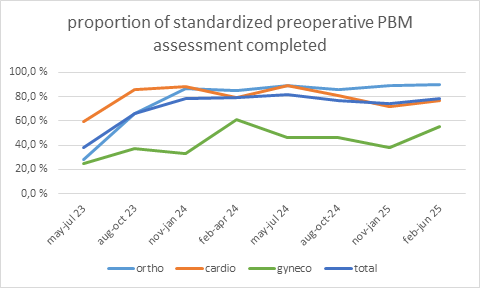
\includegraphics[width=0.85\textwidth]{figure.png}
\caption{Temporal trends of standardized preoperative PBM assessment completion rates by surgical specialty (May 2023 -- February 2025). The graph shows quarterly measurements for orthopedics (blue), cardiology (orange), gynecology (green), and overall hospital performance (dark blue).}
\label{fig:pbm_trends}
\end{figure}

\section{Discussion}

Integrating PBM indicators into a graph-based clinical data warehouse enables
 \textbf{automated quality monitoring} at hospital scale.

Our automated reports identified departments with strong adherence to specific practices 
(e.g., orthopedics for preoperative assessments) and those requiring improvement. 
These reports will serve as the primary objective outcome measure to evaluate the 
effectiveness of a micro-learning intervention targeting low-adherence specialties.

Future technical developments involve refactoring the current data stack with modern 
tools (\textbf{Dagster}, \textbf{dbt}, \textbf{OMOP}) as part of a regional clinical 
datawarehouse initiative. The objective is to replace semi-manual orchestration 
(Talend, Python scripts) with fully automated, web-accessible dashboards enabling 
real-time monitoring across the region.
\begin{thebibliography}{99}

\bibitem{shander2022global}
Shander A, Hardy JF, Ozawa S, Farmer SL, Hofmann A, Frank SM, Kor DJ, Faraoni D, Freedman J. A global definition of patient blood management. Anesthesia \& Analgesia. 2022;135(3):476--488.

\bibitem{theissen2024perioperative}
Theissen A, Folléa G, Garban F, Carlier M, Pontone S, Lassale B, Boyer B, Noll E, Arthuis C, Ducloy-Bouthors AS, et al. Perioperative patient blood management (excluding obstetrics): guidelines from the French National Authority for Health. Anaesthesia Critical Care \& Pain Medicine. 2024;43(5):101404.

\bibitem{tibi2021sts}
Tibi P, McClure RS, Huang J, Baker RA, Fitzgerald D, Mazer CD, Stone M, Chu D, Stammers AH, Dickinson T, et al. STS/SCA/AmSECT/SABM update to the clinical practice guidelines on patient blood management. The Journal of ExtraCorporeal Technology. 2021;53(2):97--124.

\bibitem{godonReductionRedBlood2024}
Godon A, Dupuis M, Amdaa S, Pevet G, Girard E, Fiard G, Sourd D, Bosson JL, Payen JF, Albaladejo P, Bouzat P. Reduction of red blood cell transfusion with a patient blood management protocol in urological and visceral surgery: A before-after study. Anaesthesia Critical Care \& Pain Medicine. 2024 Aug;43(4):101395.

\bibitem{Rabiei2022}
Rabiei R, Almasi S. Requirements and challenges of hospital dashboards: a systematic literature review. BMC Medical Informatics and Decision Making. 2022;22:287.

\bibitem{Artemova2019}
Artemova S, Madiot PE, Moreau-Gaudry A, et al. PREDIMED: Clinical Data Warehouse of Grenoble Alpes University Hospital. In: MEDINFO 2019: Health and Wellbeing e-Networks for All. 2019. p. 1421--1425.

\bibitem{Mehra2015}
Mehra T, Seifert B, Spahn DR. Implementation of a patient blood management monitoring and feedback program significantly reduces transfusions and costs. Transfusion. 2015;55:2807--2815.

\end{thebibliography}

\end{document}